\subsection{Software: KIT Head package}
\label{sec:kithead}

The Karlsruhe humanoid head~\cite{Asfour2008KITHead} was acquired as the testbed for active gaze strategies. Fig.~\ref{fig:kit_head} shows a picture of the real device.

\begin{figure}
\centering
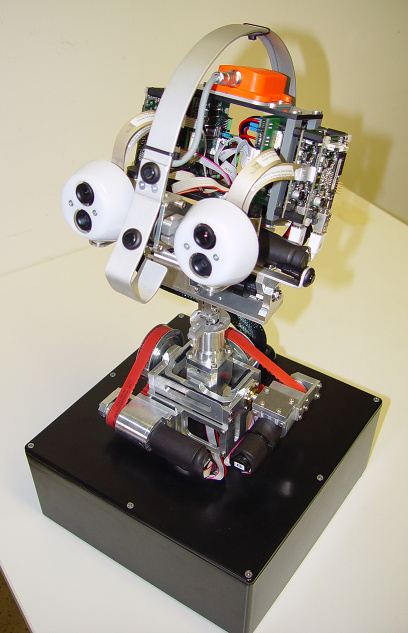
\includegraphics[width=0.25\textwidth]{kithead.png}
\caption{The Karlsruhe humanoid head.}
\label{fig:kit_head}
\end{figure}

\subsubsection{Hardware interface}

The real hardware interface is still under development. The simulated hardware interface considers the default behavior of a robot using position controlled motors. This is good enough for the planning and simulation environment, specially to test active gaze control. In order to do that, we added the simulation of point cloud acquisition, as well as two RGB cameras per eye to be as close as possible to what the KIT head offers. The simulation of the cameras is described next.

\subsubsection{Camera simulation}
There are out-of-the-box camera plug-ins for both kind of cameras, RGB and RGB-D. Both are used in the simulated head. The point cloud and images are published in an uncalibrated frame as well as in the real robot could be. Real calibration values can be loaded to have camera and robot  under the same tree of connectivity. Parameters such as noise and noise type can be set to test active gaze control and object recognition in ideal and not so ideal conditions. Fig.~\ref{fig:kit_vision} shows the simulated RGB and RGB-D cameras mounted on the eyes and forehead. Note that, the robot model has been set to almost transparent in the visualizer at the bottom, and the point cloud is overlaid covering the hand and wrist.

\begin{figure}[h!]
\centering
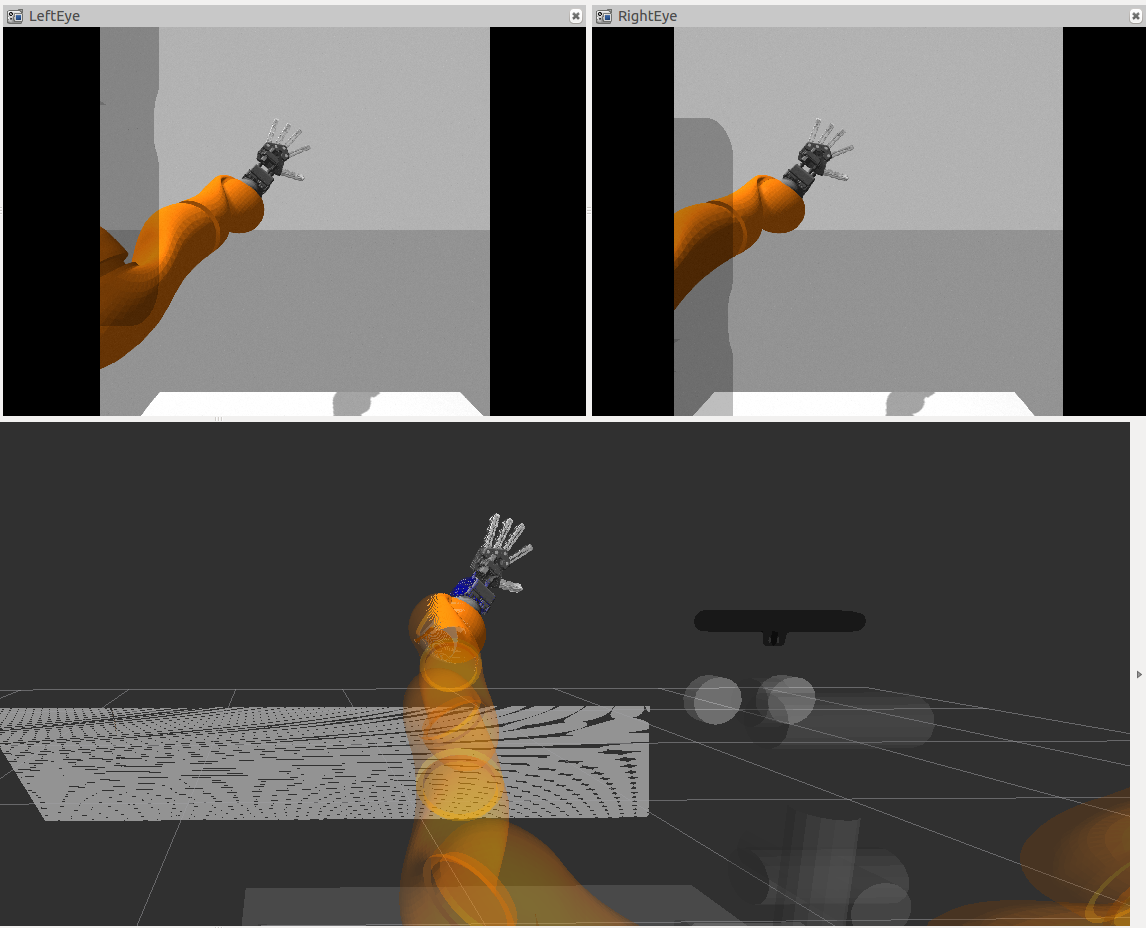
\includegraphics[width=0.7\textwidth]{headVision.png}
\caption{Simulation of RGB (top) and RGB-D (bottom) cameras available in the KIT head.}
\label{fig:kit_vision}
\end{figure}